\section{Modelos de crescimento liderados pelos gastos autônomos não criadores de capacidade}\label{Literatura}

Da seção anterior, destacou-se o o supermultuplicador sraffiano (SMS) enquanto um modelo adequado para tratar dos gastos autônomos não criadores de capacidade produtiva.
Até então, pode-se dizer que a teoria do crescimento liderado pela demanda enfrentava um dilema. Não conseguia conciliar estabilidade, distribuição funcional da renda exógena e grau de utilização da capacidade produtiva igual ao normal/planejado, aparentando uma trindade impossível do crescimento, conforme pode ser visto no diagrama \ref{diagrama}\footnote{Este diagrama é inspirado no ``trilema'' do crescimento apresentado por \textcite{cesaratto_neo-kaleckian_2015}.}.
Essa trindade impossível se mostrou falsa com o desenvolvimento do supermultiplicador sraffiano.


\begin{figure}[htb]
	\caption{Trindidade ``impossível''}
	\label{diagrama}
	\begin{center}
		\resizebox{0.45\textwidth}{!}{%
			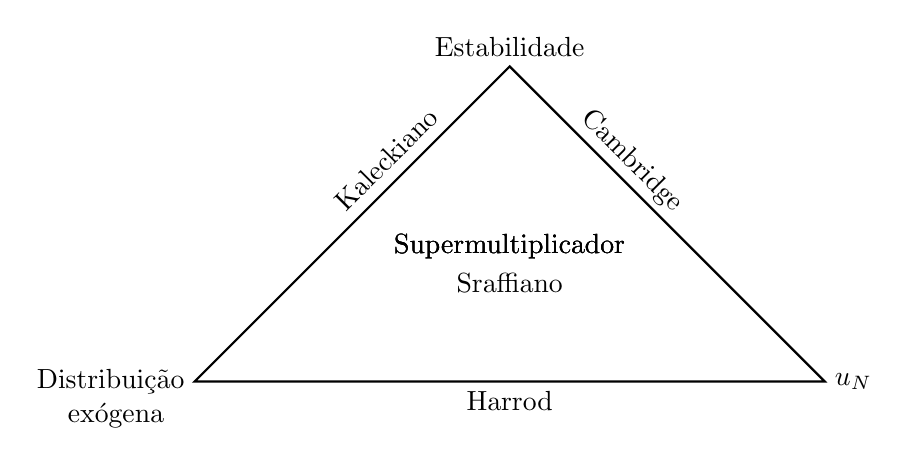
\begin{tikzpicture}[thick]
			\path[draw] (-4,0)  coordinate [label= left:Distribuição] (A)
			
			-- ( 0,4)  coordinate [label=above:Estabilidade] (C)
			-- ( 4,0)  coordinate [label=right:$u_N$] (B)
			-- cycle;
			\foreach \point in {A,B,C}
			\draw
			-- (0,2) node[anchor=north]{Supermultiplicador};
			\draw
			-- (-5,-0.15) node[anchor=north]{exógena};
			\draw
			-- (0,1.5) node[anchor=north]{Sraffiano};
			\draw
			-- (-1.75,3) node[anchor=north, rotate=45]{Kaleckiano};
			\draw
			-- (1.75,3) node[anchor=north, rotate=-45]{Cambridge};
			\draw
			-- (0,0) node[anchor=north]{Harrod};
			\end{tikzpicture}
		}
	\end{center}
	\caption*{\textbf{Fonte:} Elaboração própria}
\end{figure}

No entanto, da revisão da literatura verifica-se que tal mérito não se restringe ao SMS uma vez que uma vertente kaleckiana tem incluído tais gastos por meio do princípio do ajuste do estoque de capital no \textbf{longo prazo}.
Dito isso, esta seção pretende discutir tais desdobramentos bem como esclarecer algumas questões envolvendo a autonomia dos gastos ditos ``improdutivos'' e as respectivas controvérsias.

\section{Modelos de crescimento e os gastos autônomos: uma revisão empírica}
\label{RevF}

O objetivo desta seção é analisar os trabalhos empíricos que analisam a relação entre os gastos autônomos não criadores de capacidade produtiva ao setor privado e crescimento econômico e, assim, complementar a discussão teórica realizada na seção \ref{SecAutonomos}. Mais uma vez, seguindo a categorização de \textcite{cesaratto_technical_2003}, os referidos gastos são:
(i) consumo financiado por crédito ou riqueza acumulada;
(ii) gastos do governo;
(iii) investimento residencial;
(iv) exportações e;
(v) gastos com P\&D\footnote{
	%TODO Nota de rodapé sobre gastos com P\&D
	Nota de rodapé sobre gastos com P\&D?
}. 
Da revisão da literatura empírica, verificou-se três principais preocupações: 
\begin{description}
	\item[(a)] testar a importância dos gastos autônomos sobre a taxa de crescimento de longo prazo; 
	\item[(b)] avaliar a relação entre taxa de investimento e produto;
	\item[(c)] investigar a dinâmica de cada um dos gastos autônomos referidos anteriormente.
\end{description}
Cada um desses pontos será analisado adiante. Por fim, vale pontuar que, dados os objetivos desta investigação, serão privilegiados os trabalhos que tenham o supermultiplicador sraffiano desenvolvido por \textcite{serrano_long_1995} e \textcite{bortis_institutions_1996} como forma de análise.

No que diz respeito ao tema (a), o trabalho de \textcite{girardi_long-run_2016} se destaca por analisar os efeitos de longo prazo dos gastos autônomos sobre o produto bem como por apresentar uma forma de se calcular o supermultiplicador para a economia norte-americana. Para tanto, estimam um VECM e obtém os resultados esperados de acordo com a teoria\footnote{Mais precisamente, tais resultados se sustentam uma vez desconsiderado o consumo financiado por crédito. Como justificativa para tal medida, \textcite[p.~13]{girardi_long-run_2016} argumentam que tal gasto está associado a algumas fases do ciclo econômico e, portanto, apresenta uma parcela consideravelmente induzida.}: (i) gastos autônomos e o produto apresentam uma tendência de longo prazo (são cointegradas); (ii) relação de causalidade parte dos gastos autônomos para o produto e (iii) relação positiva entre taxa de crescimento dos gastos autônomos e taxa de investimento. Já no artigo de \textcite{girardi_autonomous_2018}, o mesmo é feito para alguns países da zona do euro com a diferença que foram utilizadas variáveis instrumentais como \textit{proxy} de alguns gastos autônomos e foram obtidos resultados semelhantes ao do estudo anterior. Por fim, o trabalho de \textcite{goes_supermultiplier_2018} possui semelhanças com o de \textcite{girardi_long-run_2016}, mas se distingue por extendê-lo para mais países e por adotar critérios para agrupá-los bem como por reportar a convergência do grau de utilização ao nível normal.

Os trabalhos empíricos envolvendo o supermultiplicador, no entanto, não estão restringidos aos EUA ou países da OCDE. \textcite{freitas_pattern_2013}, por exemplo, analisam o caso brasileiro para os anos de 1970 a 2005 e concluem que diferentes gastos autônomos (em ordem, gastos do governo e consumo financiado por crédito) lideraram o crescimento em momentos distintos. Paralelamente, \textcite{braga_investment_2018} investiga o efeito acelerador para o caso brasileiro de 1996 a 2017 e conclui que o investimento criador de capacidade produtiva é causado (no sentido de Granger) pelo produto, ou seja, é induzido.  

Enquanto \textcite{freitas_pattern_2013} e \textcite{girardi_autonomous_2015} abordam a importância dos gastos autônomos para o crescimento, \textcite{braga_investment_2018} avalia a relação entre taxa de investimento e crescimento. Assim, estão abarcadas as preocupações (a) e (b) elencadas anteriormente. Resta, portanto, evidenciar os trabalhos que destacam a importância de alguns gastos autônomos em específico. Um deles é o de \textcite{medici_cointegration_2011} em que avalia o caso argentino para os anos de 1980 a 2007 e encontra evidências de cointegração entre renda, consumo do governo e o consumo privado autônomo (\textit{i.e.} não assalariado) em que os últimos granger-causam o primeiro. O modelo apresentado por \textcite{deleidi_mission-oriented_2019}, por sua vez, também analisa a importância dos gastos do governo investigando se o tipo de política fiscal adotada tem impactos sobre o crescimento. Em linhas gerais, os autores concluem que gastos orientados em setores mais intensivos em P\&D e em mudanças estrutuais (correspondente ao gasto v) possuem efeitos maiores do que uma política centrada apenas em incentivos fiscais. Já no que diz respeito às exportações (gasto iv), destaca-se a literatura de restrição por balanço de pagamentos seguindo a lei de \textcite{mccombie_balance--payments_1994} 
%TODO Orig year Thirwall
em que as exportações são os determinantes do crescimento de longo prazo \cites{atesoglu_balance--payments-constrained_1993}{mccombie_empirics_1997}{moreno-brid_mexicos_1999}{bertola_balance--payments-constrained_2002}\footnote{Por mais que tal abordagem não lance mão explicitamente do modelo do supermultiplicador sraffiano, as conclusões são compatíveis uma vez que estão presentes gastos autônomos não criadores de capacidade e a especificação da função investimento pode seguir o princípio do ajuste do estoque de capital.}.

%======================== Investimento residencial: Arestis e gasto induzido

Por fim, no que tange o investimento residencial, verifica-se uma lacuna na literatura empírica heterodoxa de crescimento liderado pela demanda. Vale retomar a compatibilidade deste componente da demanda com o modelo do supermultiplicador uma vez que (i) não cria   capacidade produtiva ao setor privado e (ii) pelas hipotecas serem a principal forma de financiamento (e não salários) de acordo com o \textit{Survey of Construction} \cite{us_census_bureau_characteristics_2017}. Dito isso, caberá a seção seguinte examinar as formas que a literatura econométrica encontrou para incorporar o investimento residencial para então eleger uma alternativa compatível com o supermultiplicador sraffiano.
\subsection{Um breve mapeamento da fronteira heterodoxa}
\label{Hibridos}


Ao longo desta seção, serão mapeados os modelos de crescimento, 
sejam eles kaleckianos ou sraffianos, liderados pelos gastos autônomos não criadores de capacidade produtiva ao setor privado. Isso não implica que são os únicos modelos com gastos autônomos, mas sim, que são os modelos em que a participação destes gastos não converge a zero\footnote{
	No que diz respeito ao consumo financiado por crédito, por exemplo, destacam-se os trabalhos de \textcite{dutt_maturity_2006}, \textcite{palley_inside_2010} e \textcite{hein_finance-dominated_2012}.
	No entanto, esses autores trabalham no arcabouço kaleckiano básico. Por isso, a estabilidade só é garantida se o consumo financiado por crédito a crescer a mesma taxa que a acumulação --- ou seja, este componente do consumo não pode ser tratado como de fato um gasto autônomo.
	%Diante desta limitação, \textcite{pariboni_household_2016} argumenta que os gastos autônomos desempenham um papel passivo e sugere uma alternativa a partir do supermultiplicador sraffiano. 
}.
Dado que estes modelos partem do fechamento do supermultiplicador sraffiano no longo prazo, os resultados esperados são: (i) mudanças na distribuição de renda não afetam a taxa de crescimento do produto; (ii) o mesmo vale para as alterações na propensão marginal propensão a poupar; (ii) convergência do grau de utilização ao normal; (iv) taxa de crescimento da economia converge à taxa dos gastos autônomos.
Sendo assim, as especificidades de cada modelo serão explicitadas somente se os resultados anteriores se alterarem de modo que serão analisadas as implicações da inclusão dos referidos gastos autônomos na medida que contribuam para os objetivos dessa pesquisa.
%Para manter a comparatividade entre os modelos apresentados, serão realçados alguns dos resultados de \textbf{longo prazo}, são eles: (i) mudanças na distribuição de renda; (ii) alterações na propensão marginal propensão a poupar; (ii) convergência do grau de utilização ao normal; (iv) aumento da taxa de crescimento dos gastos autônomos. Por fim, as variáveis serão adaptadas de modo que $\gamma$ é o componente autônomo do investimento,  $z$ é a participação dos gastos autônomos ($Z$) na renda que crescem a taxa $g_Z$.
Feitas essas ressalvas e seguindo a tipologia de \textcite{cesaratto_technical_2003} e a categorização de \textcite{serrano_sraffian_1995}, tais gastos autônomos são: (i) gastos do governo; (ii) consumo financiado por crédito; (iii) Investimento residencial; e (iv) Exportações.


%% Modelo Allain
%TODO Comparar com a versão do artigo dele
No já mencionado modelo de \textcite{allain_tackling_2015}, os gastos não criadores de capacidade produtiva são os gastos do governo e são financiados por impostos que se ajustam endogenamente para manter o saldo primário equilibrado\footnote{
	Dentre os resultados particulares do modelo de \textcite{allain_tackling_2015}, pontuam-se os efeitos contra-cíclicos do gasto público sobre o nível de atividade e seu papel enquanto estabilizador automático do crescimento.
}.  
\textcite{hein_autonomous_2018}, por sua vez, critica este modelo por não incluir uma discussão sobre a dinâmica do \textit{déficit} e da dívida pública no longo prazo. 
Sendo assim, insere o fechamento de \textcite{allain_tackling_2015} no arcabouço contábil da metodologia SFC de modo que os gastos do governo passam a ser financiados por crédito e emissão monetária. Como consequência, \textcite{hein_autonomous_2018} afirma que este modelo passa a incluir o paradoxo da dívida, ou seja, redução da dívida pública como resultado de um aumento dos gastos do governo dado o aumento do consumo a partir da riqueza financeira. 
Dito isso, cabe realçar que neste modelo em particular, um aumento na taxa de crescimento dos gastos do governo afeta positivamente o grau de utilização que, por sua vez, não converge ao normal\footnote{
	Vale mencionar que uma das peculiaridades deste modelo é a endogeinização da distribuição funcional da renda pelo grau de utilização. No entanto, tal resultado pode decorrer da diferenciação feita por \textcite{hein_autonomous_2018} entre renda decorrente da produção e renda financeira.
}.
Tal resultado por ser visualizado por meio do grau de utilização no médio prazo que, por sua vez, não converge ao normal inclusive no longo prazo tal como na equação apresentada por \textcite[p.~326]{hein_autonomous_2018}:
\begin{equation}
\label{Eq_Hein}
u^* = \frac{g_Z - \gamma}{\gamma_u}
\end{equation}
em que $g_Z$ é a taxa de crescimento dos gastos do governo, $\gamma$ representa os \textit{animal spirits} e $\gamma_u$ é a parcela induzida do investimento das firmas.
Em linhas gerais, a equação \ref{Eq_Hein} indica que o grau de utilização não converge ao normal.
No entanto, se os gastos autônomos crescerem a uma mesma taxa que o valor do \textit{animal spirits}, o grau de utilização será nulo.
Como a estabilidade deste modelo independe de $\gamma$, não existem restrições para esse parâmetro de modo que possa zerar o grau de utilização. Dito isso, conclui-se que esta equação de \textcite[p.~326]{hein_autonomous_2018} pode estar incompleta e, assim, não se sabe o resultado particular reportado acima decorre desta especificação do grau de utilização diferente em relação ao modelo de \textcite{allain_tackling_2015} retomada abaixo
$$
u^* = \frac{g_Z - \gamma}{\gamma_u} + u_n
$$

%MODELO BROCHIER (2018): RIQUEZA FINANCEIRA ACUMULADA
Outro modelo SFC é o de \textcite{brochier_supermultiplier_2018} em que o gasto autônomo é o consumo financiado pela riqueza acumulada\footnote{
	Outro modelo com consumo a ser destacado é o de \textcite{nah_role_2019} %NAH E LAVOIE (2019): INFLAÇÃO E DISTRIBUIÇÃO ENDÓGENA
	que inclui inflação por conflito distributivo. Por mais que tal modelo apresente gastos autônomos como os demais nesta seção, a endogeinização da distribuição de renda elimina uma das hipóteses compartilhadas entre os modelos analisados e, portanto, compromete a comparação e por isso optou-se por não apresentá-lo em maiores detalhes.
}. 
Por mais que este modelo parta do fechamento do supermultiplicador sraffiano,
mudanças na distribuição impactam a taxa de crescimento de longo prazo, sendo um resultado particular deste modelo enquanto os demais resultados esperados são preservados: (i) aumento na propensão marginal a consumir a partir da riqueza acumulada aumenta a taxa de crescimento de longo prazo e; 
	(ii) grau de utilização converge ao normal.
Neste modelo, portanto, os paradoxos dos custos e da parcimônia são mantidos --- apesar dos mecanismos causais não estarem claros dado o grau de endogeneidade do sistema --- inclusive com o grau de utilização convergindo ao normal, configurando uma possível exceção ao que foi exposto até então.

%REVER

%No entanto, a menção anterior ao governo não é ocasional. MIMEO argumentam que a presença do governo no modelo atua como a geração de um gasto autônomo que persiste enquanto efeito riqueza. Desse modo, a reformulação deste modelo para uma economia sem governo gera os resultados esperados tais como aqueles apresentados anteriormente: (i) mudanças na distribuição de renda não afetam a taxa de acumulação; (ii) o mesmo vale para a propensão marginal a poupar (via propensão marginal a consumir a partir dos salários); (iii) grau de utilização converge ao desejado; (iv) mudanças na propensão marginal a consumir a partir da riqueza acumulada não alteram a taxa de acumulação. Portanto, feitas essas modificações, os resultados apresentados anteriormente são restaurados e as exceções são eliminadas\footnote{Outra modificação verificada por MIMEO é o desenho da política fiscal e, tal como na retirado do governo, alteram os resultados obtidos na simulação.}.

%TODO: Evidenciar que os resultados diferentes da Lídia não estão no modelo do Mandarino


%TESE MANDARINO: CONSUMO FINANCIADO POR CRÉDITO
Outro modelo na linha do anterior é o de \textcite{mandarino_financing_2018} em que o consumo dos trabalhadores é financiado por crédito --- adicionando um tratamento das relações financeiras ao modelo de \textcite{pariboni_household_2016} e de \textcite{fagundes_dinamica_2017} --- e obtém os resultados de longo prazo esperados dado o fechamento do supermultiplicador sraffiano (não há retornos aos paradoxos kaleckianos).
Vale destacar que este modelo é centrado nas condições de estabilidade do endividamento dos trabalhadores no longo prazo e conclui que aumentos da taxa de crescimento dos gastos autônomos, bem como na taxa de juros, implicam diminuição da taxa de endividamento dos trabalhadores e das firmas. 
Em outras palavras, tal como em \textcite{hein_autonomous_2018}, o modelo de \textcite{mandarino_financing_2018} apresenta o paradoxo da dívida.


%MODELO NAH AND LAVOIE: EXPORTAÇÃO
Analisados o consumo autônomo (financiado por crédito e riqueza) e os gastos do governo, restam os demais componentes da demanda agregada.
No modelo de \textcite{nah_long-run_2017}, semelhante ao de \textcite{dejuan_hidden_2017}, as exportações desempenham o papel dos gastos autônomos. Mais especificamente, é uma proposta para estender a contribuição de \textcite{serrano_sraffian_1995} para o caso de uma economia aberta suficientemente pequena. Os resultados de longo prazo são iguais aos apresentados anteriormente e por conta disso não serão repetidos. No entanto, este modelo se destaca por tentar reconciliar os resultados do supermultiplicador sraffiano com os regimes de crescimento da literatura kaleckiana, pontuando que os efeitos sobre o nível do produto estão sujeitos à sensibilidade da taxa de câmbio real a mudanças na distribuição de renda. 

%MODELO DUTT: INOVAÇÃO
% \textcite{dutt_observations_2018} afirma que são incapazes de fazer com que o investimento (criador de capacidade produtiva) seja determinante do crescimento no longo prazo tal como em Kalecki. Para tanto, inclui um componente de crescimento que expressa o progresso tecnológico determinado autonomamente. No entanto, tal formulação não faz com que o grau de utilização convirja ao normal e que a taxa de crescimento seja determinada pelos gastos autônomos uma vez que essa nova variável afeta a capacidade produtiva no longo prazo. Para garantir as propriedades do supermultiplicador, o progresso técnico é endogeneizado pelos gastos com P\&D ($g_R$) de forma que:
%$$
%g_I + g_R = g_S
%$$
%Neste modelo, uma vez cessados os efeitos do progresso tecnológico: 
%	(i) distribuição afeta a taxa de crescimento de médio prazo apenas; 
%	(ii) propensão marginal a poupar também não afeta o crescimento, mas determina a condição de estabilidade; 
%	(iii) grau de utilização converge ao normal; 
%	(iv) taxa de crescimento converge para a taxa de crescimento dos gastos com P\&D e o resultado se preserva com mais de um gasto autônomo. 
%Portanto, partindo desta formulação, o progresso tecnológico pode determinar o ritmo de crescimento no longo prazo sem afetar o investimento.

Por mais que estes modelos consigam dar atenção para diferentes gastos autônomos, destaca-se a escassez daqueles que tratam do investimento residencial em específico. 
Sendo assim, cabe a seção seguinte avaliar como incluí-lo na agenda de pesquisa dos modelos de crescimento liderados pela demanda.



\begin{comment}
DESCARTADOS

Além disso, a inclusão deste componente de gasto revela a resolução parcial da instabilidade harrodiana\footnote{Diferentemente de \textcite{hein_harrodian_2012}, a instabilidade harrodiana é entendida como a incapacidade das expectativas sobre o grau de utilização se ajustarem na direção correta (instabilidade fundamental nos termos de \textcite{serrano_trouble_2017}) e não como o princípio do ajuste do estoque de capital.} nos modelos kaleckianos se não forem feitas modificações adicionais\footnote{Como visto, nos modelos mais convencionais a endogeneidade do grau de utilização é suficiente para contornar esse problema. As complicações mencionadas, decorrem das sofisticações dos modelos kaleckianos.}.
%INICIO EXPOSIÇÃO
Considerando, como em \textcite{amadeo_expectations_1987}, que o investimento reaja às expectativas sobre o grau de utilização ($u^e$), a função de acumulação ($g_I$) pode ser reescrita como:

\begin{equation}
\label{Kalecki_Autonomous}
g_I = \gamma + \gamma_u (u^e - u_n)
\end{equation}
em que $\gamma$ corresponde ao componente autônomo do investimento e pode ser traduzido tanto como \textit{animal spirits} quanto expectativa média da taxa de crescimento de longo prazo \cite[p.~4]{allain_macroeconomic_2014}. A justificativa da mudança da função de acumulação é por permitir tornar explícito o princípio do ajuste do estoque de capital no longo prazo. Como visto, no curto prazo o grau de utilização não é necessariamente igual ao desejado. No entanto, se as firmas ajustam o estoque de capital, 
$$
\Delta g_i = \varphi (u^e - u_n) \hspace{2cm} \varphi > 0
$$
tais expectativas devem ser revistas:

\begin{equation}
\Delta u^e = \xi (u - u^e), \hspace{3cm} \xi > 0
\end{equation}
Da mesma forma, as expectativas em relação à taxa de crescimento secular ($\gamma$) são corrigidas pelas taxas de crescimento efetivas ($g^*$), ou seja, 
\begin{equation}
\label{Autonomo_gamma}
\Delta \gamma = \phi (g^* - \gamma)
\end{equation}
em que $\phi$ indica um fator de correção positivo. Substituindo recursivamente e seguindo os procedimentos de \textcite[p.~5]{allain_macroeconomic_2014}, obtém-se:
\begin{equation}
\label{Autonomo_u}
\Delta \gamma = \phi \gamma_u (u - u^e) \Leftrightarrow \Delta g_I = \varphi (u^e - u_n), \hspace{2cm} \varphi > 0
\end{equation}

Tal equação implica na instabilidade de Harrod uma vez que há uma sobre/sub-estimação do grau de utilização que, por sua vez, se afasta cada vez mais do grau de equilíbrio. Em outras palavras, supondo que os empresários revisem a taxa de crescimento tendencial de acordo com a efetiva e se ambas se distinguirem, não existe um mecanismo que as igualem:
\begin{citation}
When the actual rate of utilization is consistently higher than the normal rate ($u^* > u_n$), this implies that the growth rate of the economy is consistently above the assessed secular growth rate of sales ($g > \gamma$). Thus, as long as entrepreneurs react to this in an adaptive way, they should eventually make a new, \textbf{higher}, assessment of the trend growth rate of
sales, thus making use of a \textbf{larger} $\gamma$ parameter in the investment function.
\cite[p.~144, grifos adicionados e variáveis adaptadas]{hein_harrodian_2012}
\end{citation}
Essa instabilidade\footnote{Vale destacar que não é necessário recorrer à mudanças nos modelos kaleckianos para incorrer em instabilidade, como pontua \textcite{dallery_kaleckian_2007}, o que não implica que todas elas são do tipo Harrodiana.}, argumentam \textcite[p.~144]{hein_harrodian_2012}, decorre do coeficiente $\gamma$ da função de investimento que deixa de ser constante na medida que o grau de utilização se afasta do normal. Nesses termos, não é paradoxal um modelo apresentar estabilidade Keynesiana e não resolver a instabilidade de Harrod. 

A razão do porquê pode ser explicitada seguindo a exposição de \textcite{hein_harrodian_2012} e \textcite{allain_macroeconomic_2014}. 


Vale ressaltar que tal resultado se verifica mesmo com a equação \ref{eqAllain} sendo idêntica à \ref{Autonomo_u}\footnote{A diferença consiste na substituição do grau de utilização efetivo pelo esperado.} como a diferença, nada trivial, da introdução dos gastos autônomos. 


Desse modo, a introdução dos gastos autônomos não criadores de capacidade é capaz de contornar a instabilidade dos modelos kaleckianos uma vez induzido investimento no longo prazo. 

\end{comment}